\section{Literature Review}
Autonomous methods to analyze music structure have seen a robust stream of development in the past two decades.
Summarizing works that focus on analyzing musical structures either from symbolic representations like MIDI files \citep{janssen2013discovering}, or from signal-based representations like audio recordings \citep{nieto2020structure, nieto2015, paulus2010audio} have detailed state of the art and limitations of automatic MSA.

\subsection{Goals of Music Structure Analysis}
In its most general sense, music structure analysis aims to understand how the constituent parts of a piece of music relate to each other and fit together as a whole.
Therefore, when faced with either musical scores or audio recordings, discovering meaningful segments and segmentations of the input media have emerged as a universal step in conducting MSA \citep{janssen2013discovering, nieto2020structure}.
Depending on the context and goal, these segments can be of different time-scales: a single note or an entire verse in a pop song can both be appropriate segments for different goals; they can be non-overlapping as in the two scenarios described above, or they can overlap as in the case of finding segments that are similar to a specific motif or pattern.
These segments and segmentations can be analyzed further either individually or comparatively, and can be used creatively.

% Cut some thing below
I’ll summarize briefly two important analysis frameworks that produces labeled segmentations in the Music Theory literature: Schenkerian Analysis \citep{schenker2001free}, and the Generative Theory of Tonal Music \citep{lerdahl1983generative}.
Schenkerian analysis assumes that there is one overarching formal organization called the Ursatz that unifies the pitch and harmonic content of a piece of music, guided by a rather rigid structural formula that emphasizes the falling diatonic line supported by common practice functional harmony. 
Here the goal of the analysis is to show a hierarchical segmentation of the symbolic representations (pitches stripped of their duration in this case), while the resulting structure is expected to conform to canonical forms \citep{schenker2001free}. 
Similarly hierarchical, the Generative Theory of Tonal Music (GTTM) rejects the idea of preconceived forms like Schenker’s Ursatz, and elevates the importance of rythem and meterical position when compared to Schenker.
Instead of relying on a preconceived concept of canonical Ursatz, GTTM employ cognitive principles to generate the hierarchical structure from individual notes, from the bottom up \citep{lerdahl1983generative}.
In other words, while both employing hierarchical structure, GTTM and Schenkerian Analysis differ by their biases: GTTM is surface driven, where Schenkerian is concept driven.
% Moving away from from the idea of hierarchical segmentation, both Set-Theory and Neo-Reimmanian theory place more emphasis of their analysis goals on finding out important relationships between musical elements. 
% Where GTTM and Schenkerian approaches promote position finding, Set-Theory and Neo-Reimmanian approaches promote pattern matching. 
% In fact, much of the automatic techniques for symbolic music analysis has the specific task of discovering segments of musical patterns, as opposed to the audio segmentation task that is typical for automatic signal-based analysis \citep{janssen2013discovering}.

More recently, MSA has been proposed to facilitate a range of different audio applications by \cite{nieto2020structure}, ranging from automatic music generation to music visualization.
Even though good segmentations could theoretically help each of these tasks, meaningful incorporation would require an inprovement in explainability.
By providing human understandable explainations to why a model produces a certain segmentation in terms of which features and training data are more influenential, adaptating the model to different use case senarios becomes possible by adjusting features and training data to steer the model's behavior.

% However the widespread utility of automatic MSA is hindered by the poor explainability of system outputs and difficulty in transferring knowledge between system designed for different tasks.

\subsection{Segmentation Principles and Methods}

\cite{paulus2010audio} identified three main principles when segmenting music: homogeneity, novelty, and repetition.
Later on, \cite{sargent2011regularity} emplo­yed a fourth principle: regularity of segments.
The first three principles proposed by \citeauthor{paulus2010audio} can be captured by a standard tool in MSA: the self-similarity matrix (SSM) \citep{foote1999visualizing}.
The SSM records the similarity between any two points in time of some relevant musical feature, resulting in a square matrix.
The size of the matrix is determined by the temporal granularity of the smallest segment possible, with finer granulartiy generating a larger matrix.
Depending on application, the temporal granularity can be fine or corase.
% They are typically beats in audio-based MSA, and 16th notes or the note with the shortest duration in symbolic MSA.
From the computed SSM of a piece of music, homogeneity will show up as blocks, novelty will show up as edges, and repetition will show up as diagonal lines.
Figure \ref{fig:ssm} shows the SSM of a 40 seconds excerpt of Tchaikovsky's Dance of the Sugar Plum Fairy.
This excerpt starts with 3 short related phrases elaborating a dominant pedal, before ending with the famous solo celeste arppegios that leads to recapitulation.  
Variations of SSM like the lag matrix \citep{goto2003lag} and the cross recurrence matrix \citep{serra2009cross} also exist and both improve discovery of repetitions.
\begin{figure}[H]
    \centering
    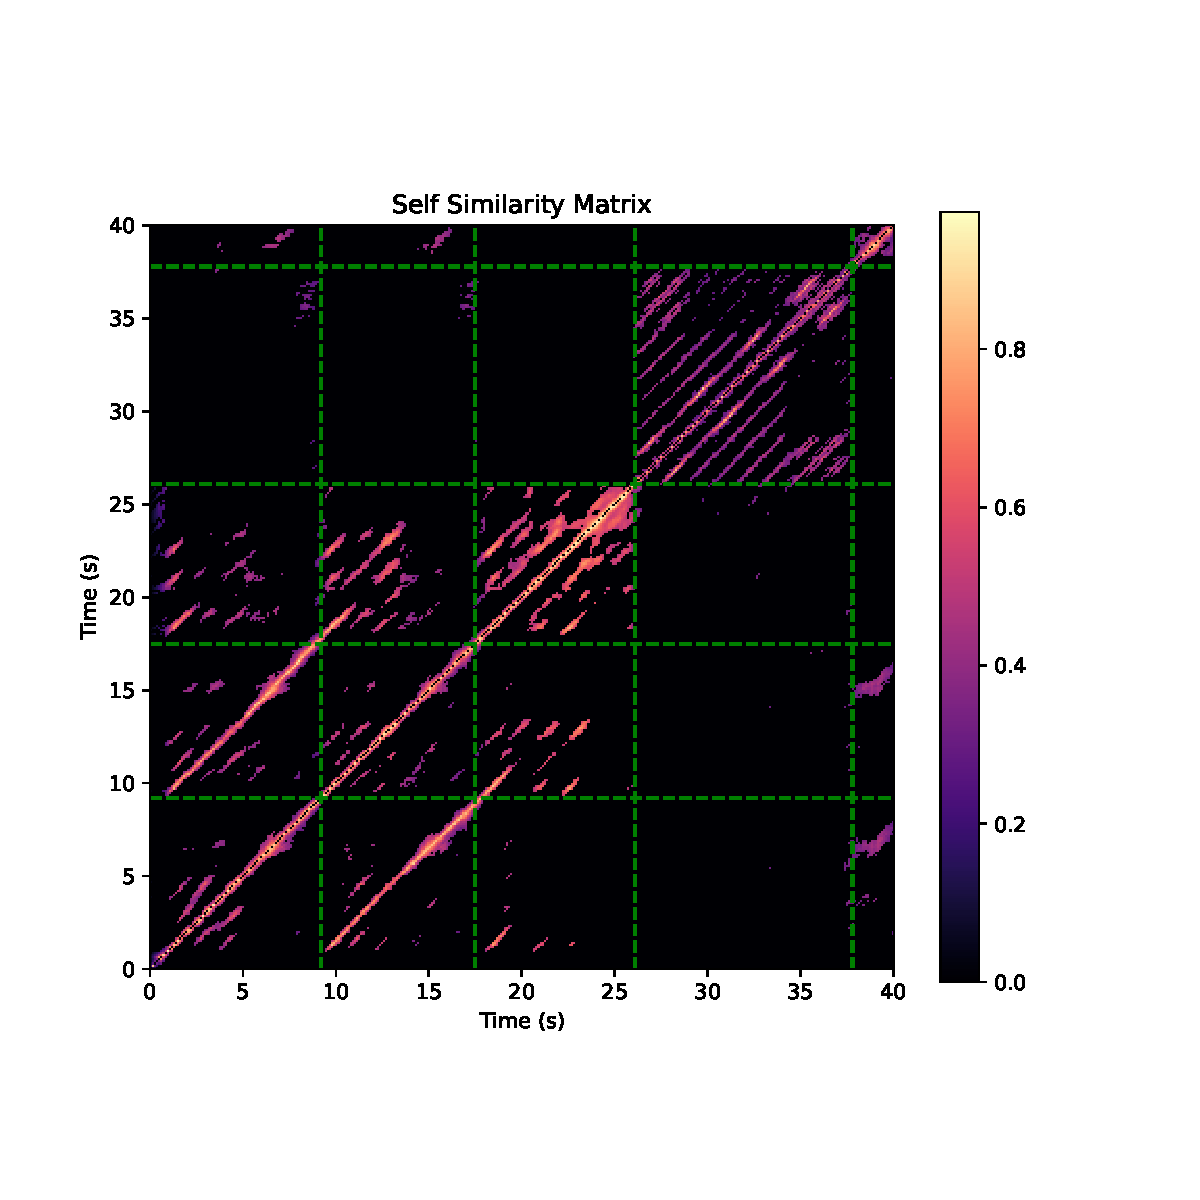
\includegraphics[height=4.5in]{ssm.pdf}
    \caption{Self Similarity Matrix of an excerpt of the Dance of the Sugar Plum Fairy by Tchaikovsky. Section boundraies are depicted by green dashed lines.}
    \label{fig:ssm}
\end{figure}

Ultimately, the structure discovered by SSM is entirely conditioned on the type of musical feature that is being examined.
While hand-crafted musical features reflecting domain knowledge are still effective \citep{mcfee2014_spectral}, features in the form of self-supervised deep neural network embeddings are start to become widespread \citep{salamon2021, mccallum2019unsupervised}.

While the SSM provide information on homogeneity, novelty, and repetition of different musical features, it still requires post-processing in general to produce segments.
Segments can be produced by convolving a checkerboard kernel along the diagonal of the SSM \citep{foote2000automatic}, which generates a novelty function that could be post-processed, for example by peak picking, to generate segment boundraies.
The relationship and similarities amongst the obtained segments and be further analyzed using techniques such as 2DMFC \citep{nieto2014}.
\cite{serra2014} achieves segmentation without convolution by shearing the SSM matrix and computing temporal flux.
Alternatively, \cite{mcfee2014_spectral} treats the segmentation problem as a clustering of musical point clouds, and applies spectral clustering using the SSM infused with temporal connectivity as the laplacian.

\subsection{Subjectivity and Hierarchy}
One of the major challenges for automatic MSA is that musical structures are highly subjective and ambiguous \citep{smith2014b}.
Part of the ambiguity in MSA comes from the hierarchical nature of musical structures, where multiple levels of segmentation of different granularity are part of the same family of heirarchically consistent segmentations, much like different levels of a Schenkerian analysis.
\cite{mcfee2017evaluating} introduces a L-measure that compares all levels of two hierarchical segmentations together, which would greatly eliminate the effect of inter-annotator discrepency due to a difference of segments temporal scale.
% More recently, the L-measure is refined and extended in works by \cite{kinnaird2021automatic}.
Beyond hierarchical ambiguity, multiple different interpretation often exists \citep{wang2017, serra2014}, which further complicates the desirable behavior of a MSA model when faced with competing interpretations.

\subsection{Explainability and Independent Musical Dimensions}
Related to the subjectivity of human structure analysis is the explainability of the outputs of automatic MSA systems.
While explainability of model outputs can be hard to measure quantitatively, \cite{molnar2019} points out several meaningful ways to provide explainbility to data-driven models.
To summarize, these methods either look at how each individual feature influecnes the overall prediciton, or they look at whether the model can associate key supportive or counterfactual data points to perticular disicions, or they could involve understanding the model's internal states or by picking inherently interpretable models like decision trees.

There has been attempts to improve MSA model explainability by looking at individual features.
\cite{smith2013quadratic} propose to study the relevance of individual musical features (e.g., rhythm, timbre, and harmony) have on the overall human production of structure annotations.
In that study, Smith and Chew posit that attentiveness to different musical dimensions may explain why two listeners disagreed about a piece's structure, and reiterate the fact that not all musical dimension contribute equally to a structure annotation of musical work.

In fact, paying attention to multiple musical dimensions independently and concurrently are highly valued by music theorists, and is termed Multivalent analysis.
\cite{webster2009multivalent}, in his book chapter on Multivalent analysis, was able to demonstrate the possibility of different musical dimension each making coherent, yet often different and contrapuntal, structures.
Webster emphasizes the need to be context sensitive in performing Multivalent analysis, and concurs with the view that prioritizing different musical dimensions is a major source of subjectivity in interpretation.
More recently, younger music theorists like \cite{brody2016parametric} and \cite{yust2018organized} have both embraced Multivalent analysis and achieved new musical insight by looking at separable musical dimensions both individually and concurrently.
Based on these trends in both MIR and music theory, I would argue that factoring musical works into separate dimensions and studying their individual structure and their contribution to different structral interpretations is a key to improve automatic MSA system's explainability.
By factoring out the analysis into musically meaningful dimensions, this approach should be promising for adapting MSA systems to different use case scenarios as well.

% \subsection{Topological Relationships}
% One attractive idea in Neo-Reimannian theory is the incorporation of geometry and topologies like the Tonnetz to explain musical similarity and distances of elements.
% Besides tonnetz, other topological spaces like the ones introduced by \cite{callender2008generalized} can also be used to compute similarity metrics, or facilitate descriptions of relationships.
% Such ideas has already seen their applications in automatic symbolic music analysis \citep{harte2006}, and the dissertation by \cite{tralie2017geometric} also showcase the potential of rigorously incorporating topological relationships has on increasing the explainability and utility of audio-based MSA.
% % In his book, \cite{yust2018organized} also dedicated 2 chapters on how graph and geometry can be used to represent and reason about temporal structures of different musical dimensions.
% These trends inspires me to incorporate topological and geometrical relationships in musical analyses, and I believe this added view point of how musical elements transition from one to another in time will be valuable to provide better model output explainability and improve adaptivity to different use cases.
